The size of the search region materially changes this comparison. Figure~\ref{fig:scaling} shows 28 independent $96^2$ media on a two-metre domain ($ka=11.85$) and seven compact $24^2$ media. For the former, at $10\%$ noise the full-aperture Born class and nonlinear peak cap 0.5 were excluded on all 28, whereas the chosen bounds excluded cap 0.75 on none. For the compact set the joint bound excluded cap five on five of seven and the material of peak 4.28 supplies a physically legal control. These are distinct data and material contracts. The compact comparison has $ka=4.27$, twelve incident fields, 48 receiving ports and $1\%$ noise; the large-domain comparison has ten fields and 20 ports. Here $a$ is the enclosing radius of the computational square. The numbers identify a limitation of unrestricted peak inference in one aperture and electrical size. They do not define a geometry-independent limiting contrast. The angular bandwidth of radiated fields is itself a scale, not a strict finite rank \cite{bucci87}.
\begin{figure}[tb]\centering
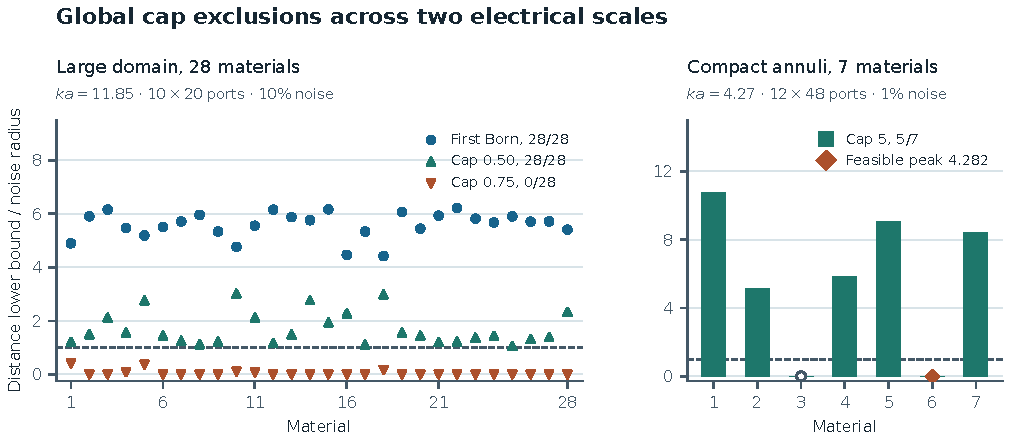
\includegraphics[width=.93\linewidth]{scaling}
\caption{Independent materials at two electrical sizes. A point above one excludes the stated hypothesis. A point at or below one measures the limit of the calculation. In the right panel one material is known to be within the proposed cap. Material indices are local to each panel.}\label{fig:scaling}
\end{figure}
